\documentclass[11pt,a4paper]{article}
\usepackage[utf8]{inputenc}
\usepackage[T1]{fontenc}
\usepackage[margin=1in]{geometry}
\usepackage{graphicx}
\usepackage{xcolor}
\usepackage{float}
\usepackage{listings}
\usepackage{upquote}
\usepackage{booktabs}
\usepackage{tcolorbox}

\lstset{
    basicstyle=\ttfamily\small,
    breaklines=true,
    frame=single,
    numbers=left,
    numberstyle=\tiny,
    backgroundcolor=\color{gray!10},
    keywordstyle=\color{blue},
    commentstyle=\color{green!50!black},
    stringstyle=\color{red},
    showstringspaces=false
}

\newtcolorbox{notebox}{colback=blue!5,colframe=blue!40!black,title=Note,fonttitle=\bfseries}

\title{\textbf{Practice 6 -- Configuring Simulator Objects}}
\author{
    Robotics and Cyber-Physical Systems \\
    School of Sciences and Engineering \\
    Tecnol\'ogico de Monterrey
}
\date{}

\begin{document}
\maketitle

\section*{Introduction}

In this activity, you will configure the simulated world without editing the
robot model or MuJoCo XML files. You will import textured objects, choose their
initial poses, change the robot's starting pose, enable a RoboCasa kitchen, and
move objects interactively.

These settings only affect the simulator. Robot programs can continue using
the same \texttt{Robot} interface on the physical and simulated robots.

\subsection*{Before You Begin}

Update the repository and its dependencies:

\begin{lstlisting}[language=bash]
git pull
git submodule update --init --recursive
uv sync
\end{lstlisting}

\section{Selecting a Configuration}

Open \texttt{sim\_config.py} in the root of the repository. This file contains
several \texttt{SimConfig} objects. The last line selects the active one:

\begin{lstlisting}[language=Python]
CONFIG = _DEFAULT
\end{lstlisting}

For example, select the Android group with:

\begin{lstlisting}[language=Python]
CONFIG = _ANDROID_ARMY
\end{lstlisting}

Every time the simulated \texttt{Robot} starts, it loads this file
automatically. Stop and restart the script after changing \texttt{CONFIG}.

\section{Importing an Object}

Each imported object needs a 3D mesh. A \texttt{texture.png} file is optional,
but gives the mesh its original colors. The included Android example uses files
from the MuJoCo Scanned Objects collection.

\begin{figure}[H]
    \centering
    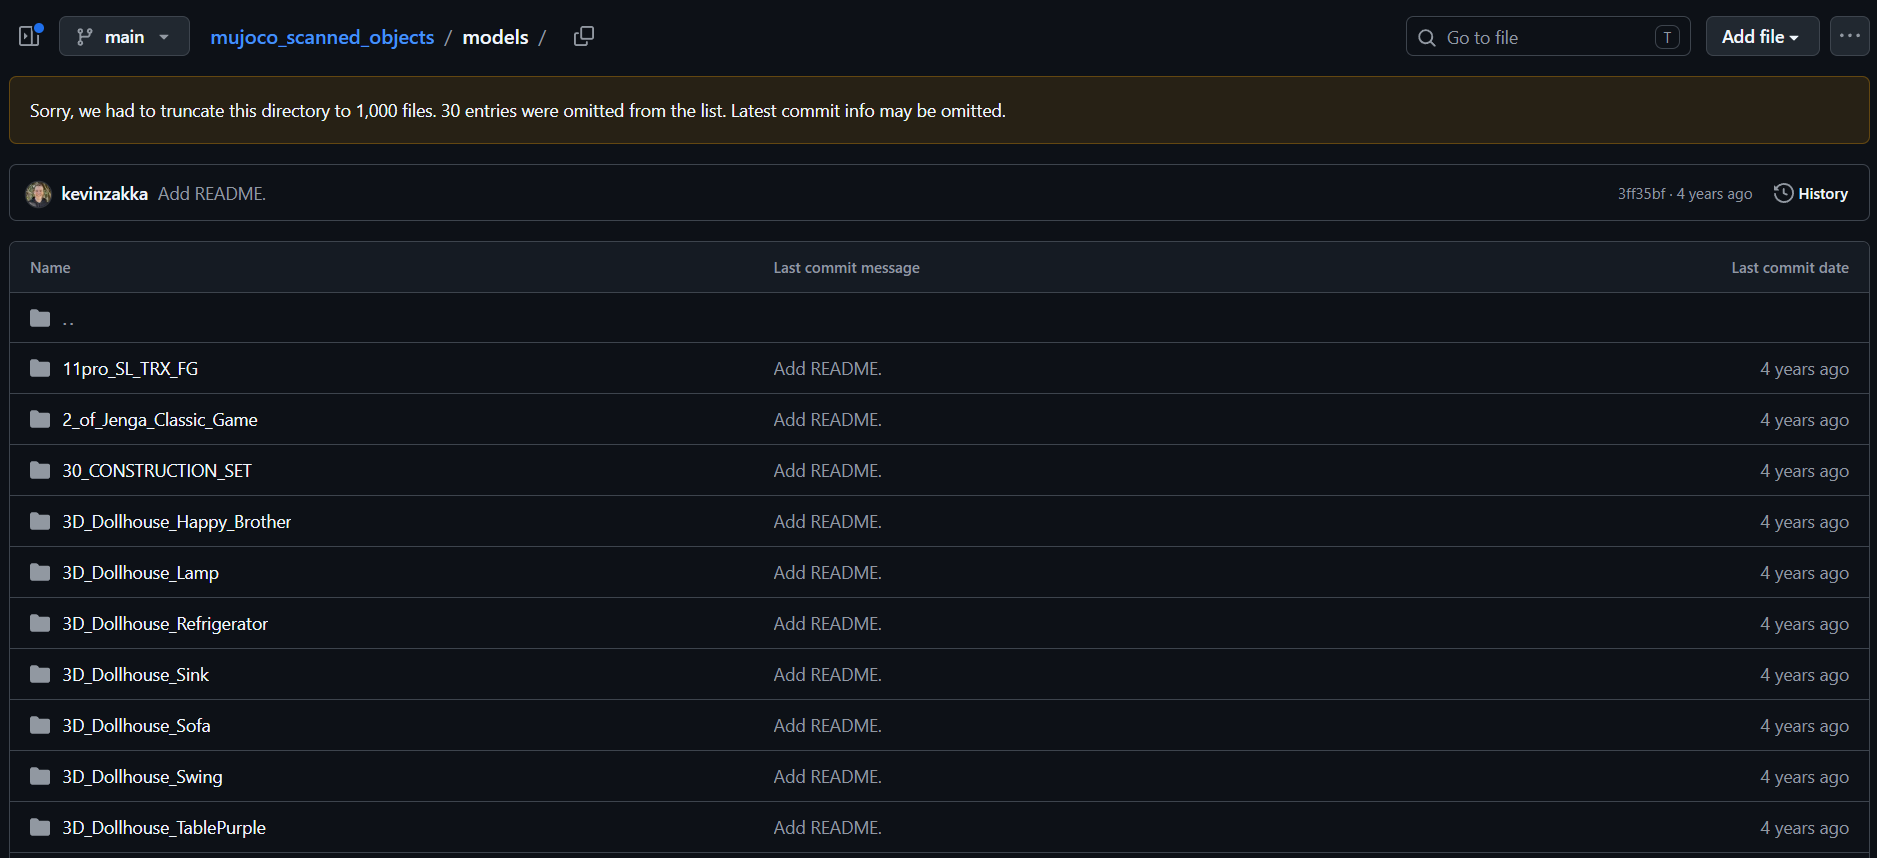
\includegraphics[width=0.75\textwidth]{mujoco_scanned_objects.png}
    \caption{Examples from the MuJoCo Scanned Objects collection.}
\end{figure}

Place an object's files in a folder inside the repository, then describe it in
\texttt{sim\_config.py}:

\begin{lstlisting}[language=Python]
_OBJECT = SimConfig(
    objects=[
        MeshObject.from_folder(
            "stretch_mujoco/models/assets/custom_objects/"
            "mujoco_scanned_objects/models/Android_Lego",
            name="configured_lego",
            position=(0.18, -0.55, 0.55),
        ),
    ],
)
\end{lstlisting}

\texttt{from\_folder()} looks for \texttt{model.obj} and
\texttt{texture.png} by default. It also estimates a box collision shape from
the mesh and calculates mass using a density of $1000\,\mathrm{kg/m^3}$.

The most useful optional arguments are:

\begin{itemize}
    \item \texttt{name}: unique name used to identify and select the object.
    \item \texttt{position=(x, y, z)}: initial world position in metres.
    \item \texttt{orientation=(w, x, y, z)}: initial quaternion.
    \item \texttt{scale=(x, y, z)}: mesh scale along each axis.
    \item \texttt{gravity}: whether gravity initially affects the object.
    \item \texttt{collision\_size}, \texttt{collision\_position},
          \texttt{mass}, and \texttt{density}: optional physics overrides.
\end{itemize}

The automatic values are good starting points. Supply the physics overrides
only if the estimated collision box or mass does not behave correctly.

\begin{figure}[H]
    \centering
    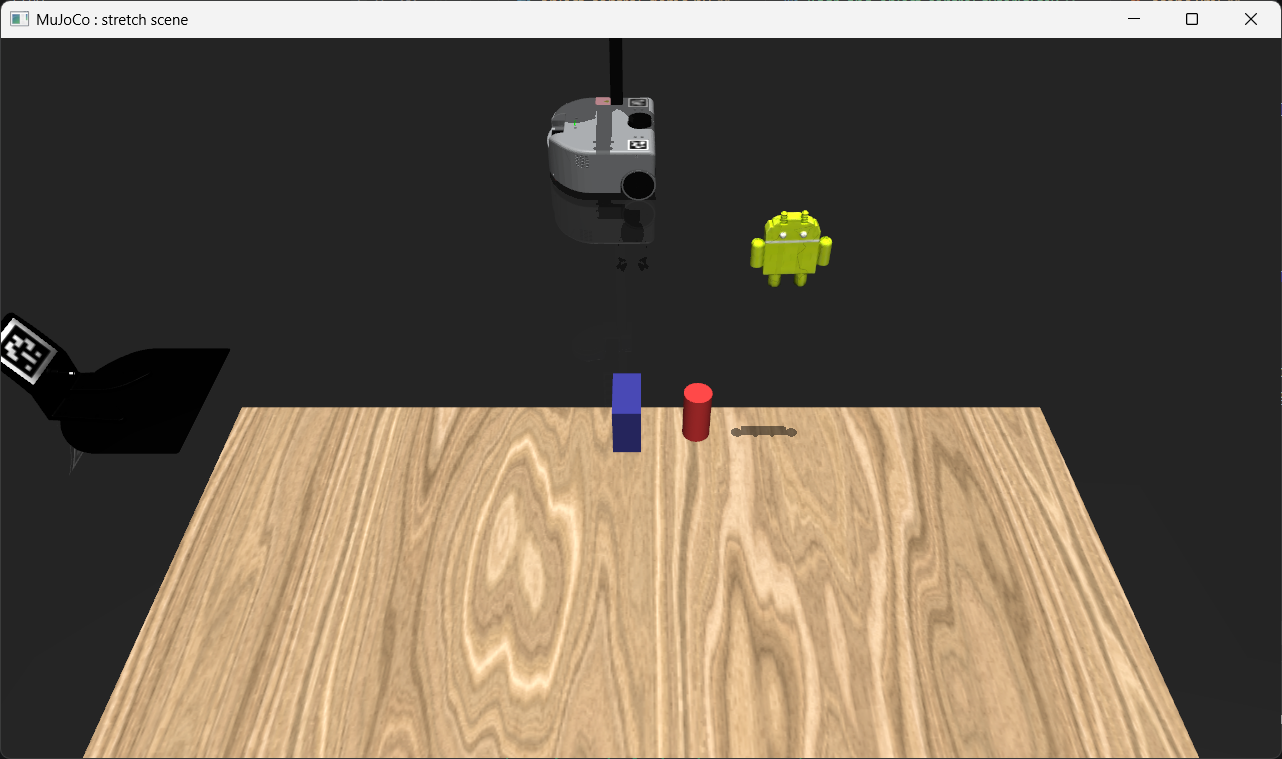
\includegraphics[width=0.72\textwidth]{android_lego_scene.png}
    \caption{A textured Android object imported into the default scene.}
\end{figure}

\subsection{Importing Several Objects}

Every object must have a unique name. A comprehension is convenient when
creating a group:

\begin{lstlisting}[language=Python]
_ANDROID_ARMY = SimConfig(
    objects=[
        MeshObject.from_folder(
            "stretch_mujoco/models/assets/custom_objects/"
            "mujoco_scanned_objects/models/Android_Lego",
            name=f"android_{row}_{column}",
            position=(0.6 + row * 0.2,
                      -0.4 + column * 0.2,
                      0.02),
            scale=(0.5, 0.5, 0.5),
        )
        for row in range(5)
        for column in range(5)
    ],
)
\end{lstlisting}

This creates 25 independently movable, half-scale Androids.

\section{Changing the Robot's Starting Pose}

Use \texttt{RobotPose} to change the simulated robot's initial world pose:

\begin{lstlisting}[language=Python]
_ROBOT_POSE = SimConfig(
    robot_pose=RobotPose(
        position=(0.5, 0.0, 0.0),
        orientation=(0.7071, 0.0, 0.0, 0.7071),
    ),
)
\end{lstlisting}

Position is expressed in metres and orientation is a quaternion in
\texttt{(w, x, y, z)} order. The example starts the robot 0.5 m from the world
origin and rotated approximately $90^\circ$ around the vertical axis.

\section{Using a RoboCasa Environment}

RoboCasa generates a furnished kitchen instead of loading the default scene:

\begin{lstlisting}[language=Python]
_ROBOCASA = SimConfig(
    robocasa=RoboCasaConfig(
        enabled=True,
        task="PnPCounterToCab",
        layout=0,
        style=0,
    ),
)
\end{lstlisting}

\texttt{task} selects the RoboCasa task, while \texttt{layout} and
\texttt{style} select the kitchen geometry and appearance.

Objects use exactly the same \texttt{MeshObject} configuration in the default
scene and in RoboCasa:

\begin{lstlisting}[language=Python]
_ROBOCASA_OBJECT = SimConfig(
    robocasa=RoboCasaConfig(
        enabled=True,
        task="PnPCounterToCab",
        layout=0,
        style=0,
    ),
    objects=[
        MeshObject.from_folder(
            "stretch_mujoco/models/assets/custom_objects/"
            "mujoco_scanned_objects/models/Android_Lego",
            position=(0.0, 0.0, 1.0),
        ),
    ],
)
\end{lstlisting}

\begin{figure}[H]
    \centering
    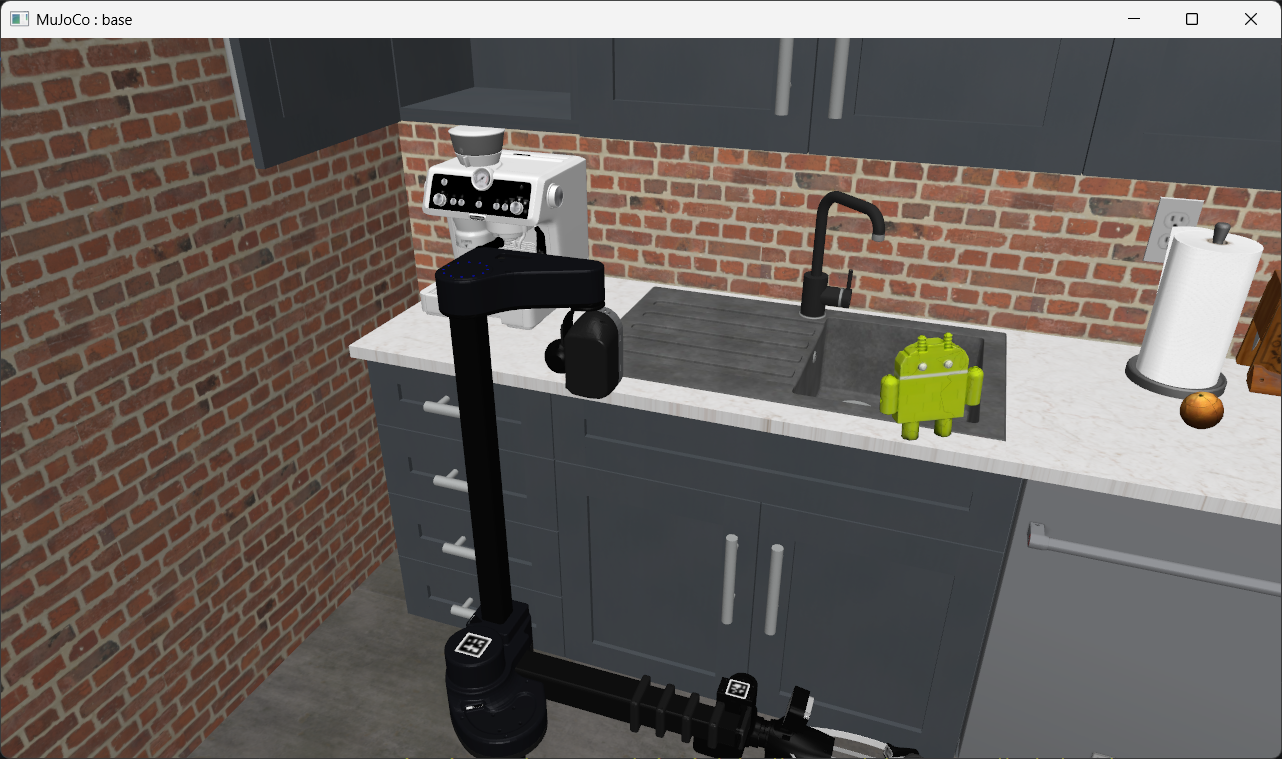
\includegraphics[width=0.72\textwidth]{robocasa_custom_object.png}
    \caption{A custom object imported into a generated RoboCasa kitchen.}
\end{figure}

\section{Moving Objects Interactively}

Object controls start automatically whenever the scene contains movable
objects. Run any simulated robot script, then press \texttt{T} to switch
between robot control and object control. No changes to the script are needed.

\begin{center}
\begin{tabular}{lll}
\toprule
\textbf{Keyboard} & \textbf{Gamepad} & \textbf{Action} \\
\midrule
\texttt{T} & START & Toggle object-control mode \\
\texttt{M} / \texttt{N} & RB / LB & Next / previous object \\
\texttt{WASD} & Left stick & Move horizontally \\
\texttt{Z} / \texttt{X} & Right stick Y & Move up / down \\
\texttt{U} / \texttt{O} & LT + right stick X & Roll \\
\texttt{I} / \texttt{K} & LT + right stick Y & Pitch \\
\texttt{J} / \texttt{L} & LT + left stick X & Yaw \\
\texttt{G} & Y & Disable gravity; object floats \\
\texttt{F} & B & Enable gravity; object falls \\
\bottomrule
\end{tabular}
\end{center}

While object mode is active, these keyboard and gamepad commands are hidden
from \texttt{TeleopProvider}. This prevents the same input from moving the
robot and an object simultaneously.

\begin{figure}[H]
    \centering
    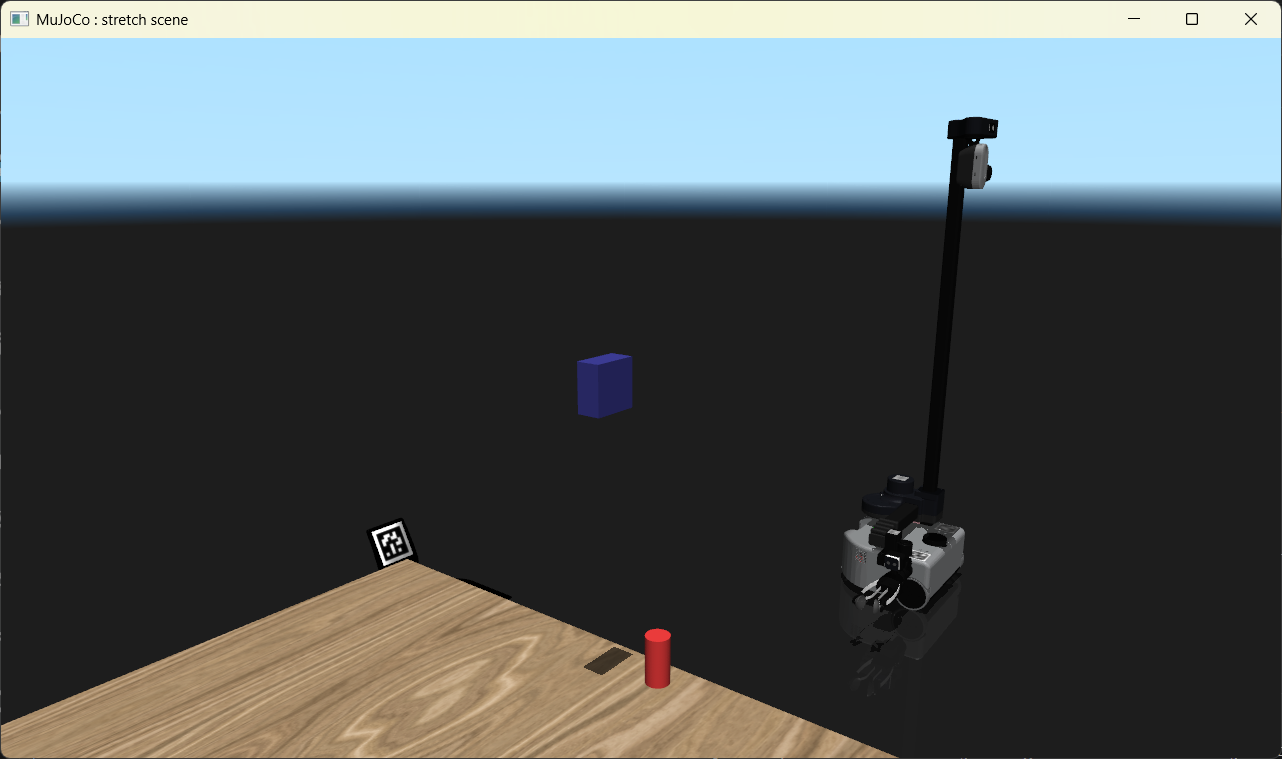
\includegraphics[width=0.72\textwidth]{object_control_demo.png}
    \caption{An object being repositioned interactively in MuJoCo.}
\end{figure}

\begin{notebox}
Disable gravity before placing an object in mid-air. Re-enable it afterward to
let the object settle naturally onto a table or the floor.
\end{notebox}

\section{Optional Programmatic Control}

Simulator-specific experiments can also access objects through
\texttt{robot.world}:

\begin{lstlisting}[language=Python]
android = robot.world.get_object("configured_lego")

print(android.position)
android.move_by(x=0.10, yaw=0.25)
android.move_to(position=(0.5, 0.0, 0.8))
android.set_gravity(False)
\end{lstlisting}

\texttt{move\_by()} applies a relative translation or rotation.
\texttt{move\_to()} assigns an absolute world pose. This API is useful for
simulator-specific tests; portable robot scripts should rely on the automatic
controls instead.

\section*{Expected Result}

You should be able to select a configuration, import one or many textured
objects, launch either the default scene or RoboCasa, and reposition every
movable object without modifying the robot-control script.

\end{document}
